\section{Methodology}
\begin{figure}[h]
  \centering
  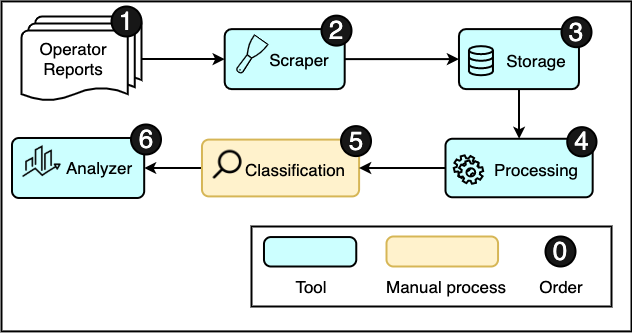
\includegraphics[scale=0.5]{diagrams/process.png}
  \caption{Data collection, extraction, and analysis process.}
  \label{fig:process diagram}
\end{figure}
Cloud providers self-report information about service availability and failures through public status pages.
We selected three of the largest worldwide cloud service providers: Amazon Web Services (AWS), Microsoft Azure, and Google Cloud Platform (GCP).
The whole workflow is shown in \autoref{fig:process diagram}.
We use data scraped from their public status pages for self-reported failures \cite{awsFeed, gcpFeed, azureFeed} in the span of one year, Jan-Dec 2018.
The pages were scraped every six hours, to avoid burdening the page host with more frequent scrapes and potentially incurring penalties (step 2 in \autoref{fig:process diagram}).
The raw dataset is approximately 522 KiB in size; the cleaned and processed dataset is around 172 KiB.

We use Python 3.7.7, Pandas 1.0.3, NumPy 1.18.4, SciPy 1.4.1, and Pytz 2019.3 to process and analyze the extracted structured failure data.
We first deduplicate the data based on the service name, failure location, and event start time, selecting the events with the longest duration (step 4 in \autoref{fig:process diagram}).
This removes 400 events in total: 137 from Azure, 127 from AWS, and 136 from GCP.
We convert all reported event start times to the timezones appropriate to the region specified for the outage.
We calculate the event duration in minutes based on the event start and end times.
We also compute the year the event took place, as well as the hour of week (with hour 0 denoting midnight on Monday).
We then filter the data, selecting events that occurred in the 2018 calendar year.
This yields a grand total of 411 events: 139 from GCP, 144 from AWS, and 128 from Azure.

The providers also include in their reports a textual description of the outage.
The description does not follow a specific format or standard, and must thus be manually analyzed for each event.
We classify outages across several categories based on the description of the outage (step 5 in \autoref{fig:process diagram}).
The classification is partially based on that done by Gunawi et al. \cite{gunawi2016, gunawi2014}, but as many of the failure descriptions are terse and brief, our classification is less detailed.

The description provides information about the qualitative aspects of the outage.
We identify seven such aspects: how many services were affected, the severity, the range, the users affected in the outage, the root cause of the outage, the duration of the outage, and the components of the service affected in the outage.
An outage can affect one or multiple services.
The severity can be visual (i.e. performance is not affected, only visual feedback is incorrect), degradation of performance, or complete unavailability of the service.
The range of an outage can be (in ascending order by geographical size) a single availability zone, a single region, or multiple regions.
As the range of a single availability zone only applies to AWS services, outages that occurred in a single availability zone (13 events) were merged with those occurring in a single region, to simplify analysis.
An outage can affect some users, or all users; this is meant to be understood in combination with the range of the outage (e.g. an outage may affect all users in a single region).
The cause of an outage can be a code error, a side effect of maintenance, a configuration error, a network error, an external factor, increased load, or an unhealthy unit.
A ``unit'' is not necessarily a physical (i.e. hardware) unit, but can be a virtual node, a cluster, etc.

Each of these causes can be further separated into narrower categories.
A configuration error can stem from a direct change to a configuration file, or can happen as part of a deployment task.
A network error can indicate an internal API issue, or an internal network issue.
An external factor can be the environmental conditions in the datacenter (e.g. higher temperatures or humidity), a shock event (e.g. a thunderstorm), or an issue caused by a third party.
If one of these features is not stated in the description of a particular outage, we note that it was not provided for the outage.
